\documentclass[12pt]{article}
\usepackage{graphicx}
\usepackage{subcaption}
\usepackage{mwe}
\usepackage[]{mcode}
%\usepackage{lingmacros}
%\usepackage{tree-dvips}
%\usepackage{blindtext}
%\usepackage[utf8]{inputenc}

\begin{document}

\title{CMSC 426 - P2}
\author{Gudjon Einar Magnusson}

\maketitle

\section{Capture Images} %1
For this project I used 5 sets of images to test my code.

\begin{figure}[t!]
    \begin{subfigure}[t]{0.3\textwidth}
        \centering
        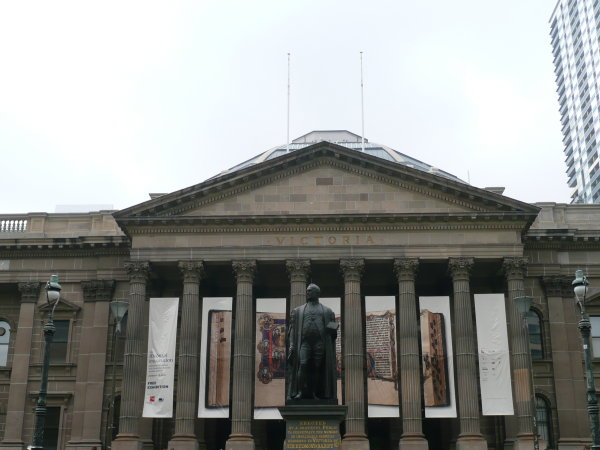
\includegraphics[width=\linewidth]{../Images/Set1/1}
    \end{subfigure}
    \begin{subfigure}[t]{0.3\textwidth}
        \centering
        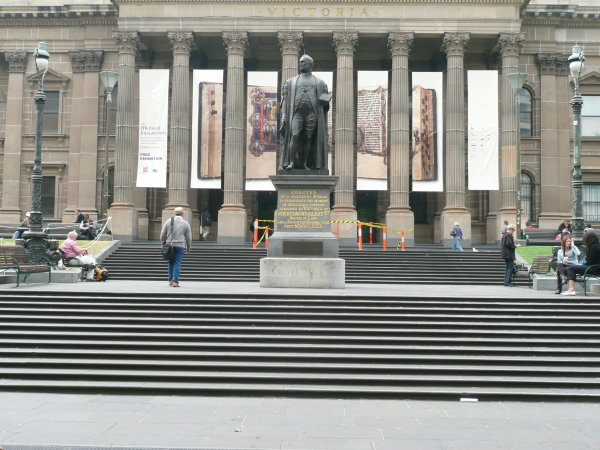
\includegraphics[width=\linewidth]{../Images/Set1/2}
    \end{subfigure}
        \begin{subfigure}[t]{0.3\textwidth}
        \centering
        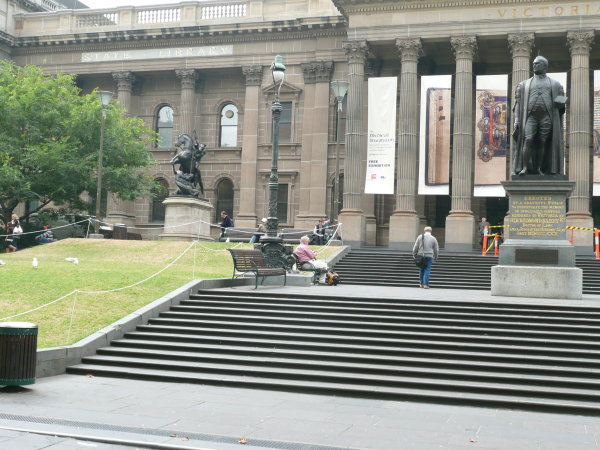
\includegraphics[width=\linewidth]{../Images/Set1/3}
    \end{subfigure}

    \vskip\baselineskip

    \begin{subfigure}[t]{0.3\textwidth}
        \centering
        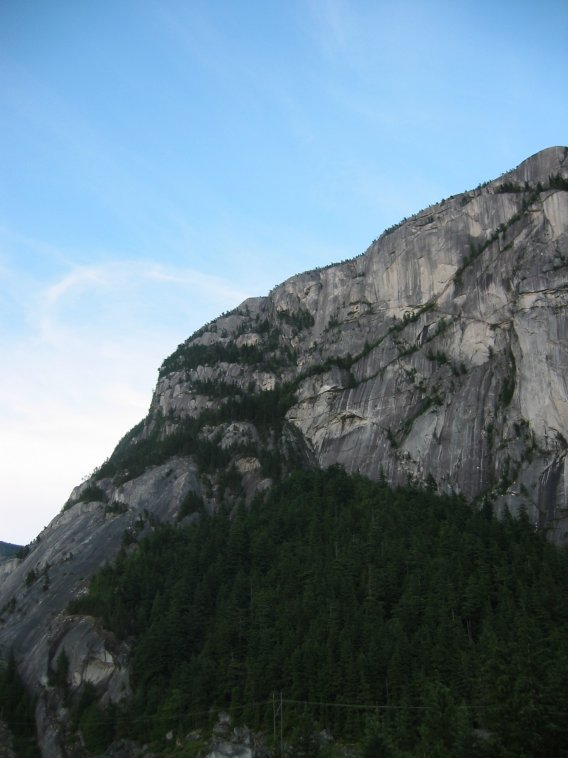
\includegraphics[width=\linewidth]{../Images/Set2/1}
    \end{subfigure}
    \begin{subfigure}[t]{0.3\textwidth}
        \centering
        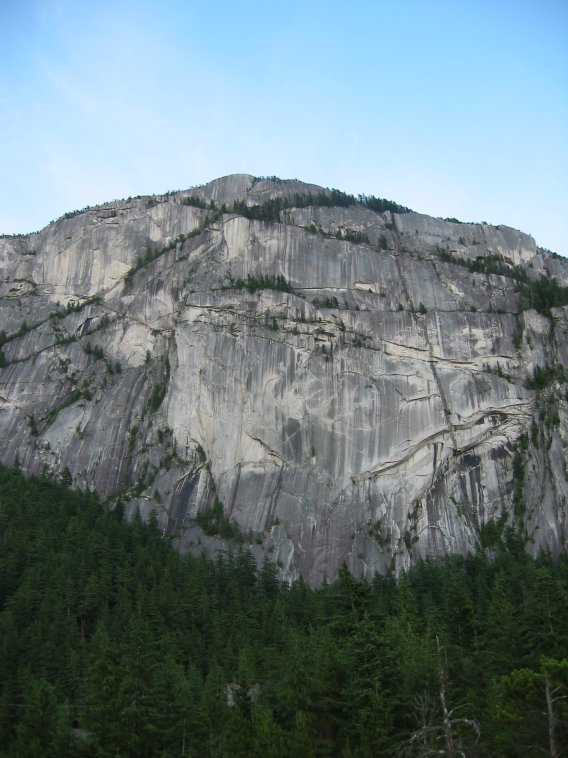
\includegraphics[width=\linewidth]{../Images/Set2/2}
    \end{subfigure}
        \begin{subfigure}[t]{0.3\textwidth}
        \centering
        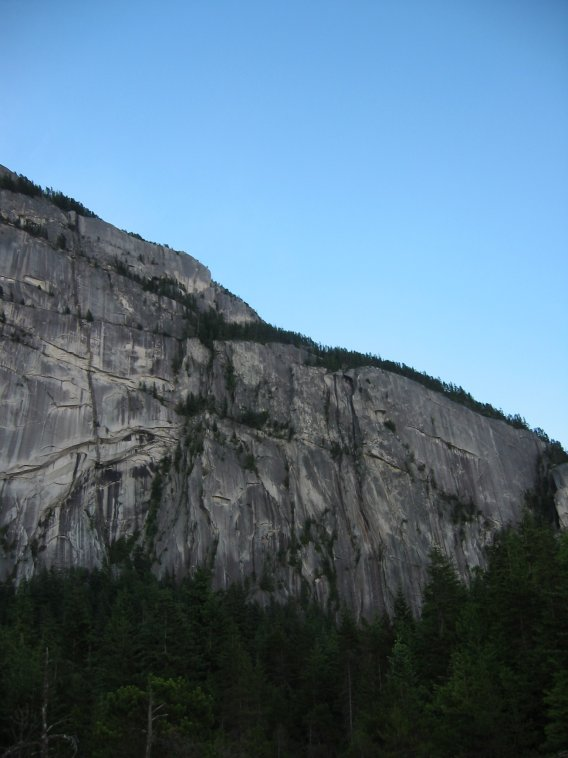
\includegraphics[width=\linewidth]{../Images/Set2/3}
    \end{subfigure}

    \vskip\baselineskip

    \begin{subfigure}[t]{0.1\textwidth}
        \centering
        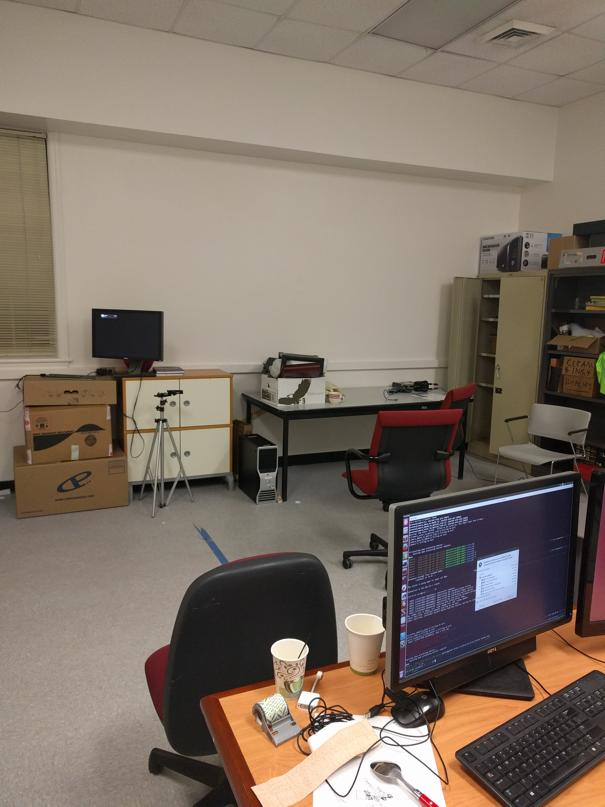
\includegraphics[width=\linewidth]{../Images/Set3/1}
    \end{subfigure}
    \begin{subfigure}[t]{0.1\textwidth}
        \centering
        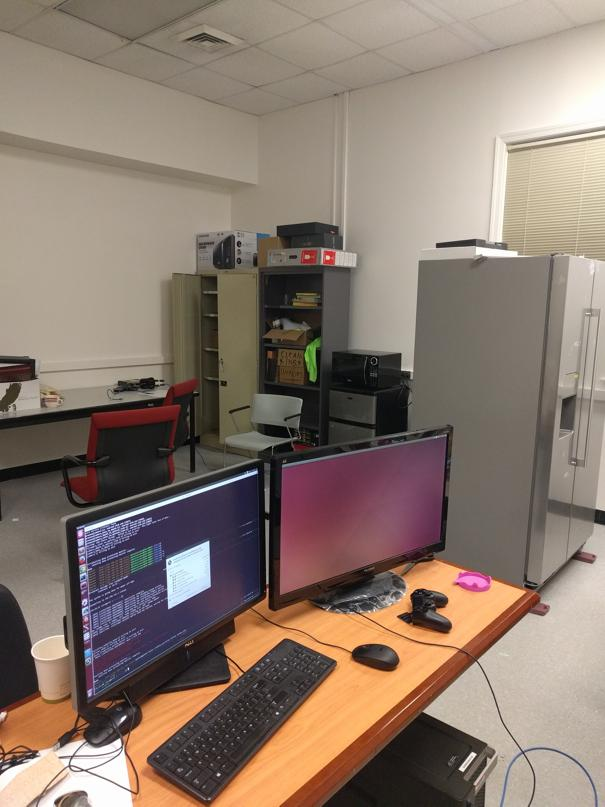
\includegraphics[width=\linewidth]{../Images/Set3/2}
    \end{subfigure}
    \begin{subfigure}[t]{0.1\textwidth}
        \centering
        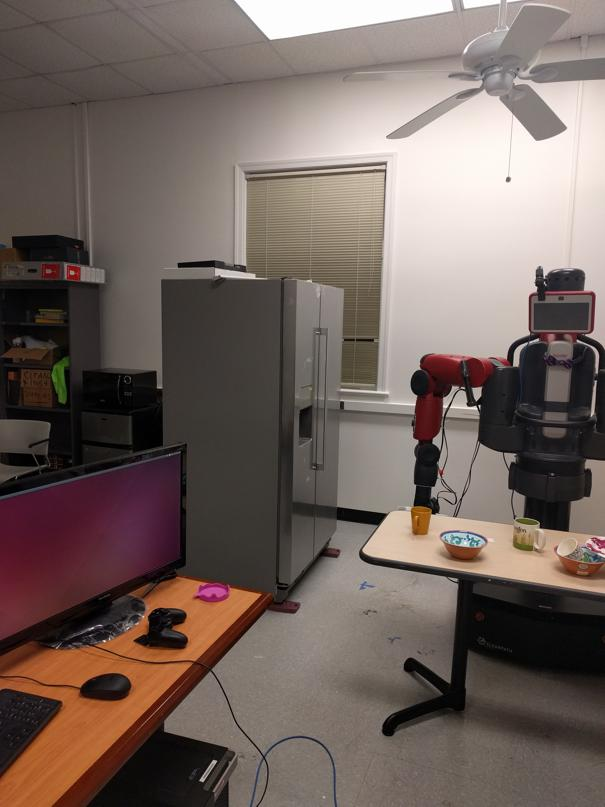
\includegraphics[width=\linewidth]{../Images/Set3/3}
    \end{subfigure}
    \begin{subfigure}[t]{0.1\textwidth}
        \centering
        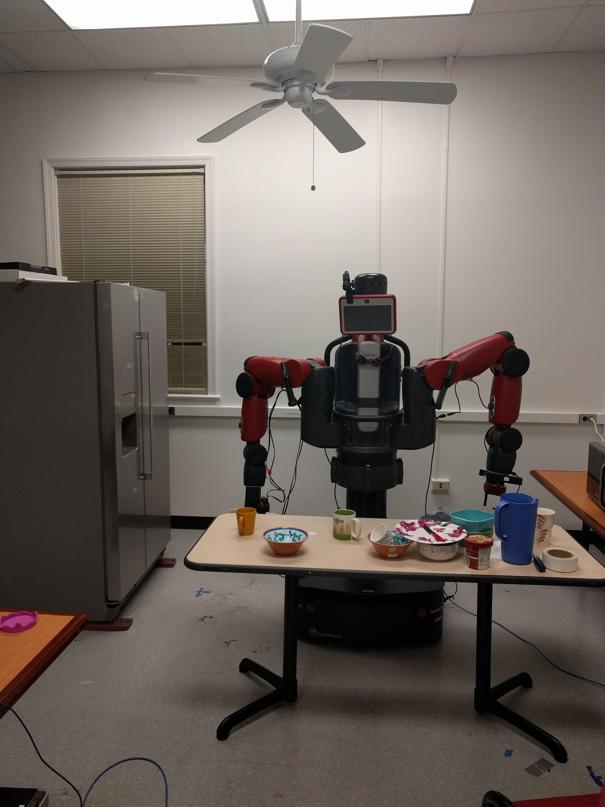
\includegraphics[width=\linewidth]{../Images/Set3/4}
    \end{subfigure}
    \begin{subfigure}[t]{0.1\textwidth}
        \centering
        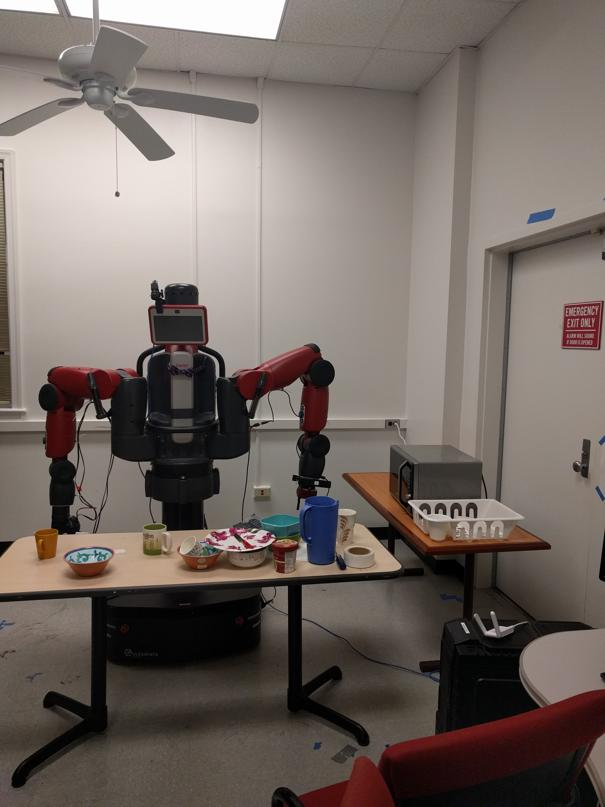
\includegraphics[width=\linewidth]{../Images/Set3/5}
    \end{subfigure}
    \begin{subfigure}[t]{0.1\textwidth}
        \centering
        
\includegraphics[width=\linewidth]{../Images/Set3/6}
    \end{subfigure}
    \begin{subfigure}[t]{0.1\textwidth}
        \centering
        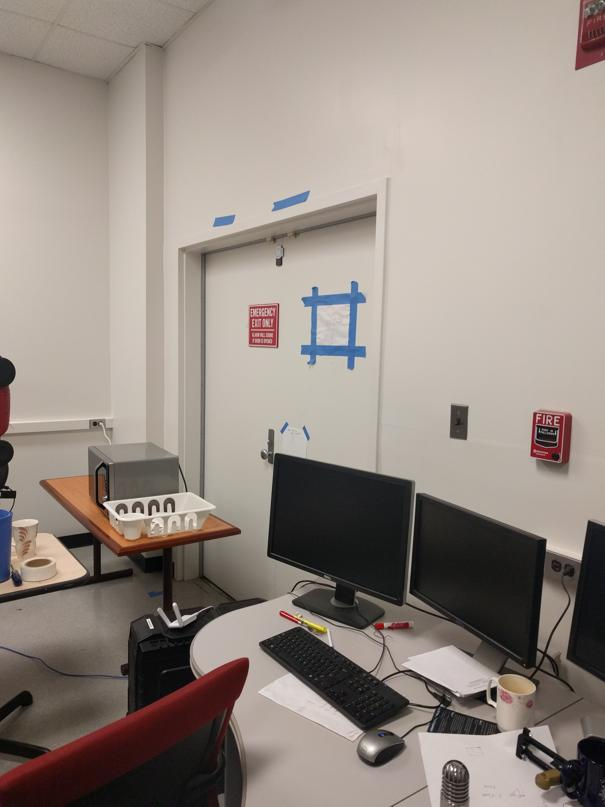
\includegraphics[width=\linewidth]{../Images/Set3/7}
    \end{subfigure}
    \begin{subfigure}[t]{0.1\textwidth}
        \centering
        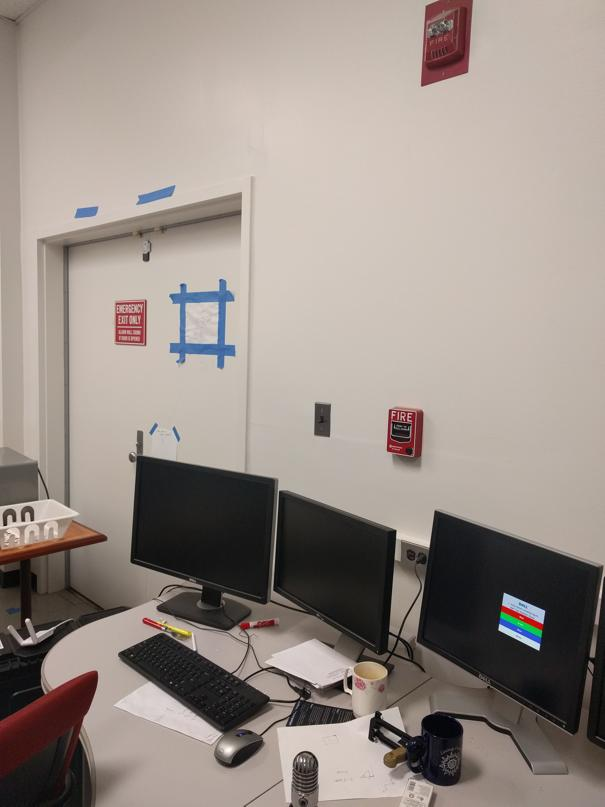
\includegraphics[width=\linewidth]{../Images/Set3/8}
    \end{subfigure}

    \vskip\baselineskip

    \begin{subfigure}[t]{0.3\textwidth}
        \centering
        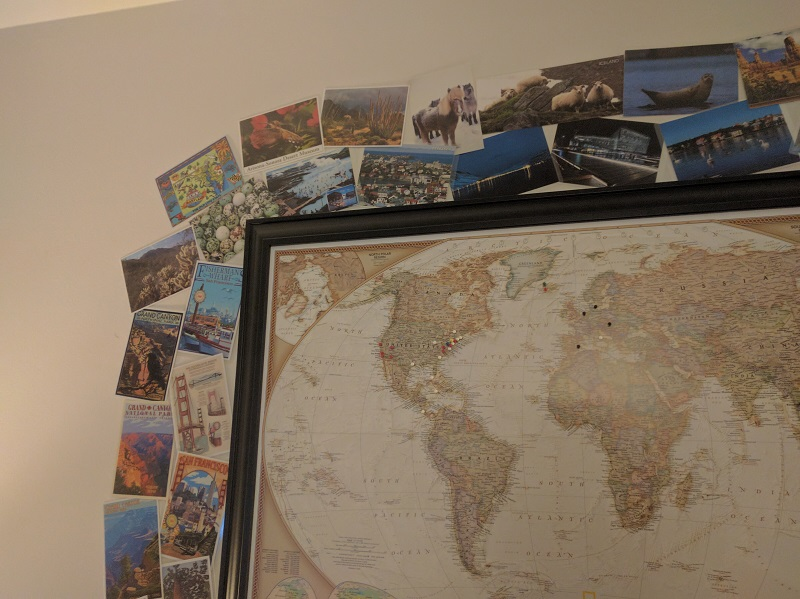
\includegraphics[width=\linewidth]{../Images/CustomSet1/1}
    \end{subfigure}
    \begin{subfigure}[t]{0.3\textwidth}
        \centering
        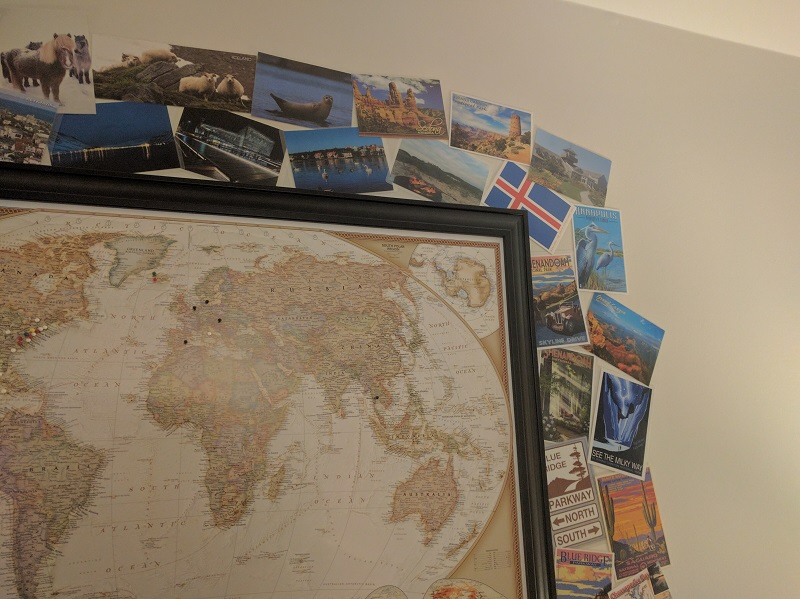
\includegraphics[width=\linewidth]{../Images/CustomSet1/2}
    \end{subfigure}
        \begin{subfigure}[t]{0.3\textwidth}
        \centering
        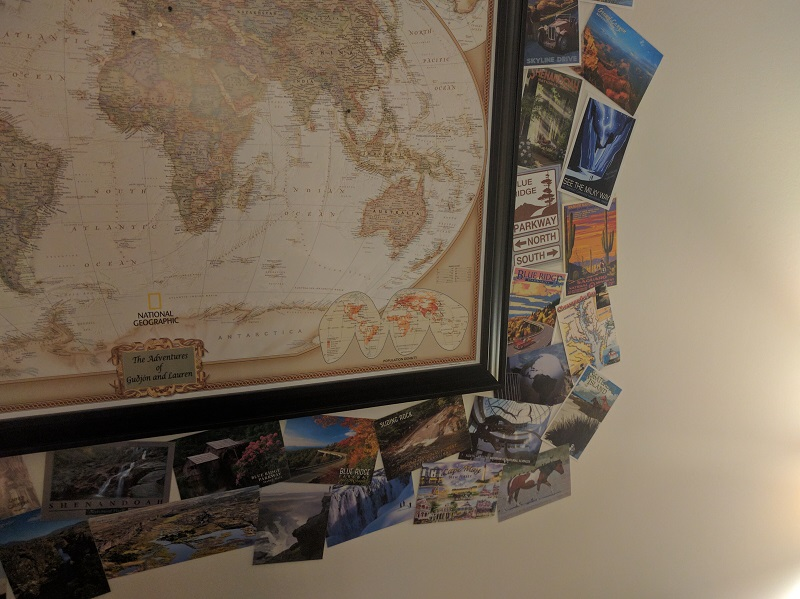
\includegraphics[width=\linewidth]{../Images/CustomSet1/3}
    \end{subfigure}

    \caption{Image set}
    \label{fig_set1}
\end{figure}


\section{Feature Correspondence} % 2

\subsection{ANMS}

The ANMS algorithm is implemented in the the function \textit{anms}. It takes two arguments, a matrix of corner metrics $C$ and the max number of corners to return, $n$. It returns two vectors, $x$ and $y$ with the coordinates of the points.

The initial set of points is picked by finding peaks in corner metric matrix using the \textit{imregionalmax} function. The points are then ranked based on their distance form other points and the top $n$ points are returned. This results in a set of points that are roughly evenly spread across the image. In my implementation I generally use $n = 300$. I tried higher values but got little benefit from it. 

\subsection{Feature Descriptor}

Feature descriptors are used to identify each corner across images. To do this I implemented the function \textit{fdescript}. I takes three arguments, an image $I$ and two vectors $r$ and $c$ with the index of the points of interest.

For each point I take the surrounding $40\times40$ pixel region and apply a Gaussian blur with sigma equal to 4. From that result I take the value from every fifth row and every fifth column, resulting in 64 values. Those values are normalized by subtracting the mean and dividing by the standard deviation. The normalized values serve as the descriptor for that corner.

\subsection{Feature Matching}

Feature matching is implemented in the function \textit{matchFeatures}. It takes four arguments, the corner coordinates and descriptor values for each of the two images we want to pair.

For every point it calculates the square difference from every other point by comparing the descriptor values. The point pair is accepted only if the difference is low and its significantly lower than the next best batch. In my implementation I only accepted the point pair if the lowest difference divided by the next lowest difference was lower than 0.3.

\subsection section{RANSAC}

The RANSAC algorithm is implemented in the function \textit{ransac}. It takes three arguments, two sets of points, $M1$ and $M2$, and the maximum number of iterations, $iter$.

\section{Output}

To put together a set of images $I$, I first estimate the homography from each image to the first image, the set of homographies is called $H$. The first homography $H_1$ is simply the identity matrix, $H_2$ is the projection from $I_2$ to $I_1$, $H_3$ is the projection from $I_3$ to $I_1$, and so on. To do this I assume that each image in the set can be matched with the one before it. Then I can project each image to the first one multiplying $H_n$ with $H_{n-1}$. 

This makes it easy to project one image after another as long as the images are given in the correct order. The problem wit this approach is that as we move further from the first image the distortion gets worse. Long panoramas look good on one end but are distorted at the other. A better way is to project all the images to the center image. To do that I multiply each homography with the inverse of the center homography. Figure \ref{fig_pan_center} shows how the choice of a center image affects the panorama.

\begin{figure}[t!]
    \begin{subfigure}[t]{0.5\textwidth}
        \centering
        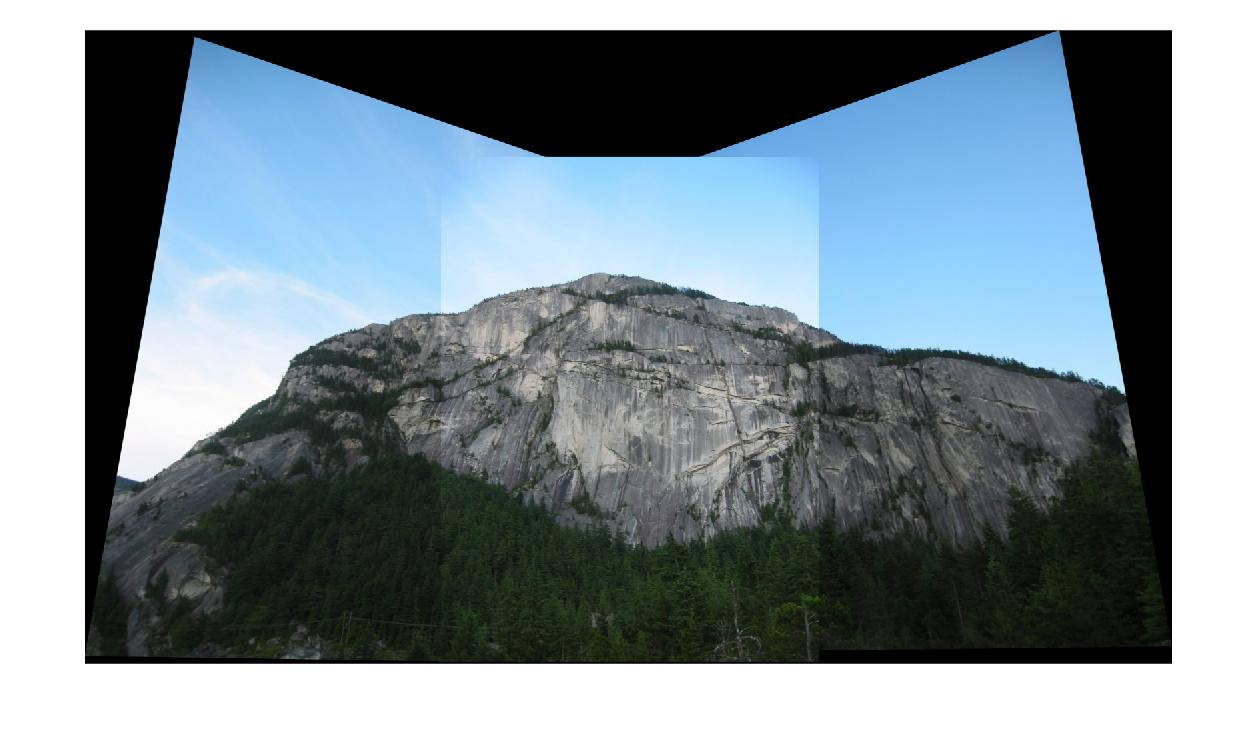
\includegraphics[width=\linewidth]{img/set2_panorama3}
        \caption{Panorama with 3 images projected to the center image}
        \label{fig_set2_pan1}
    \end{subfigure}
    \begin{subfigure}[t]{0.5\textwidth}
        \centering
        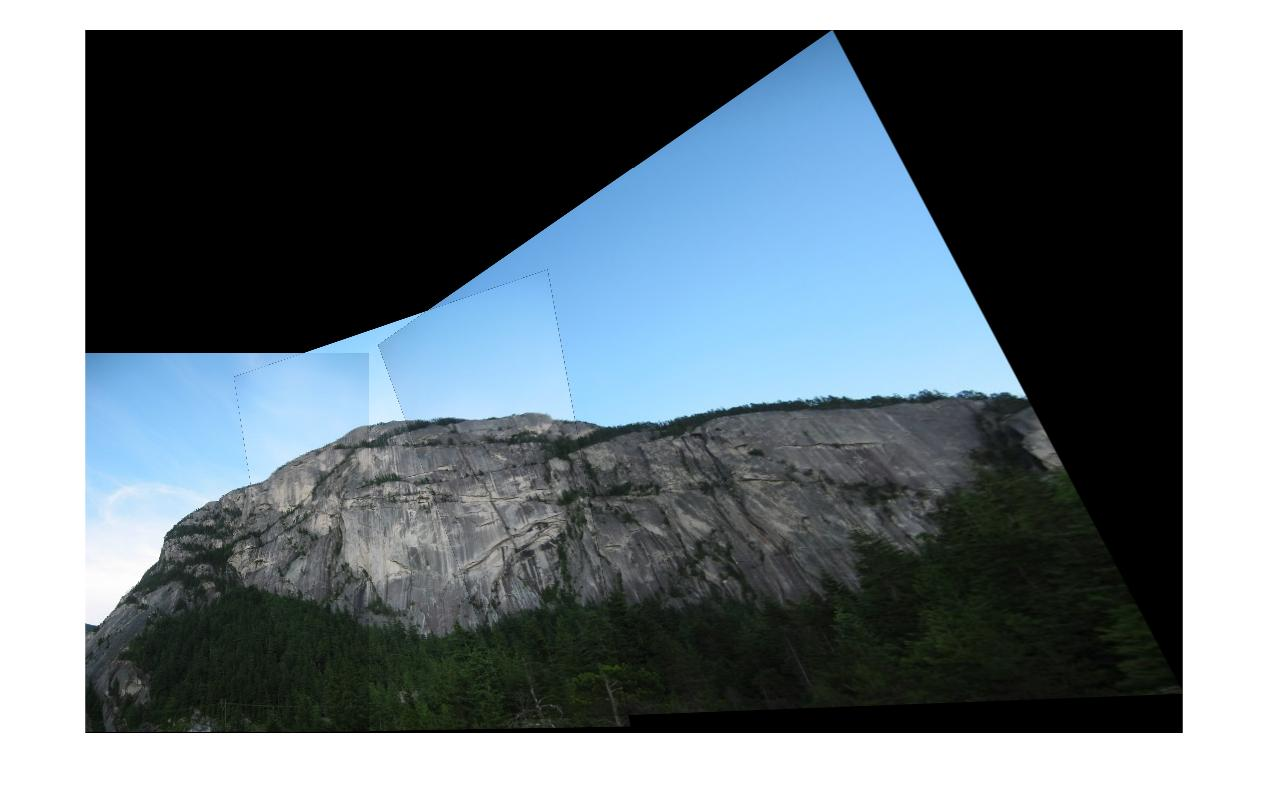
\includegraphics[width=\linewidth]{img/set2_panorama2}
        \caption{Panorama with 3 images projected to the first image}
        \label{fig_set2_pan2}
    \end{subfigure}
    \caption{Picking a good center makes the panorama much better}
    \label{fig_pan_center}
\end{figure}

To transform a set of images once I have the homography I implemented the function \textit{transformSet}. It takes two arguments, a set of images $I$ and a set of homographies $H$. It returns a set of transformed images and a set of binary masks that shows what pixels the images occupy.

The transformation is implemented using the built in Matlab functions \textit{maketform} and \textit{imtransform}. 


\section{Cylindrical Projection}

Cylindrical projection is implemented in the function \textit{cylindrical}. It takes two arguments, an image $I$ and focal length $f$, and return another image $C$ that is the same size as $I$. When mapping pixels from the source image to the their destination confidante I simply use floor of $x'$ and $y'$. Figure \ref{fig_cyl_proj} shows and example of the output of from \textit{cylindrical}.

Lower values of $f$ increase the amount of warping in the image, kinda like lowering the radius of the cylinder that the image is projected on.

\begin{figure}[t!]
    \begin{subfigure}[t]{0.5\textwidth}
        \centering
        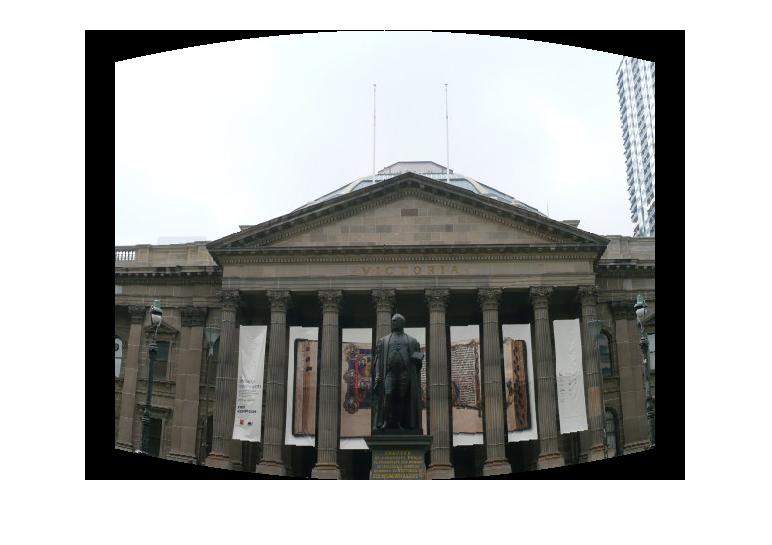
\includegraphics[width=\linewidth]{img/cylinder3}
        \caption{Cylindrical projection with $f = 500$}
        \label{fig_cyl_proj1}
    \end{subfigure}
    \begin{subfigure}[t]{0.5\textwidth}
        \centering
        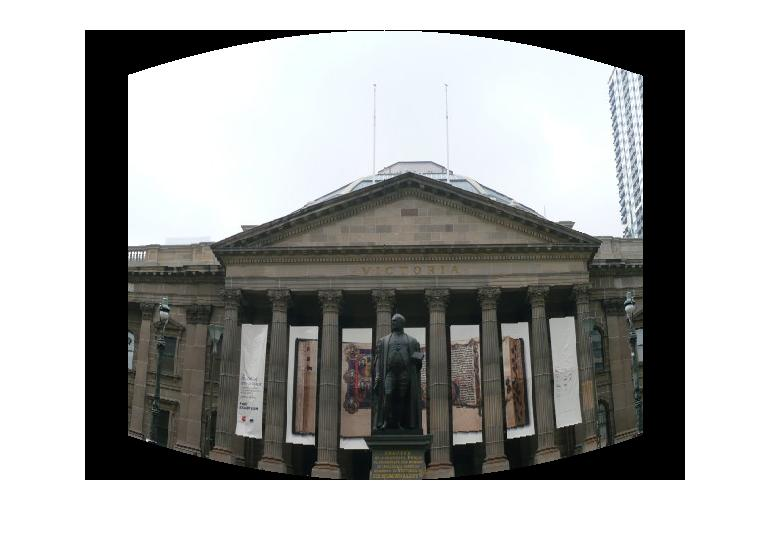
\includegraphics[width=\linewidth]{img/cylinder4}
        \caption{Cylindrical projection with $f = 400$}
        \label{fig_cyl_proj2}
    \end{subfigure}
    \caption{Examples of cylindrical projection}
    \label{fig_cyl_proj}
\end{figure}


\section{Blending}

The simplest method I could come up with to combine the image was to pick the maximum value of each pixel. This produces a fairly good result for the landscape image, except for a slight difference in brightness. For scenes closer to the camera there is a big problem, objects that move or don't match perfectly show up as ghosts. Figure \ref{fig_ghost} shows an example of the ghosting effect.

\begin{figure}[t!]
    \centering
    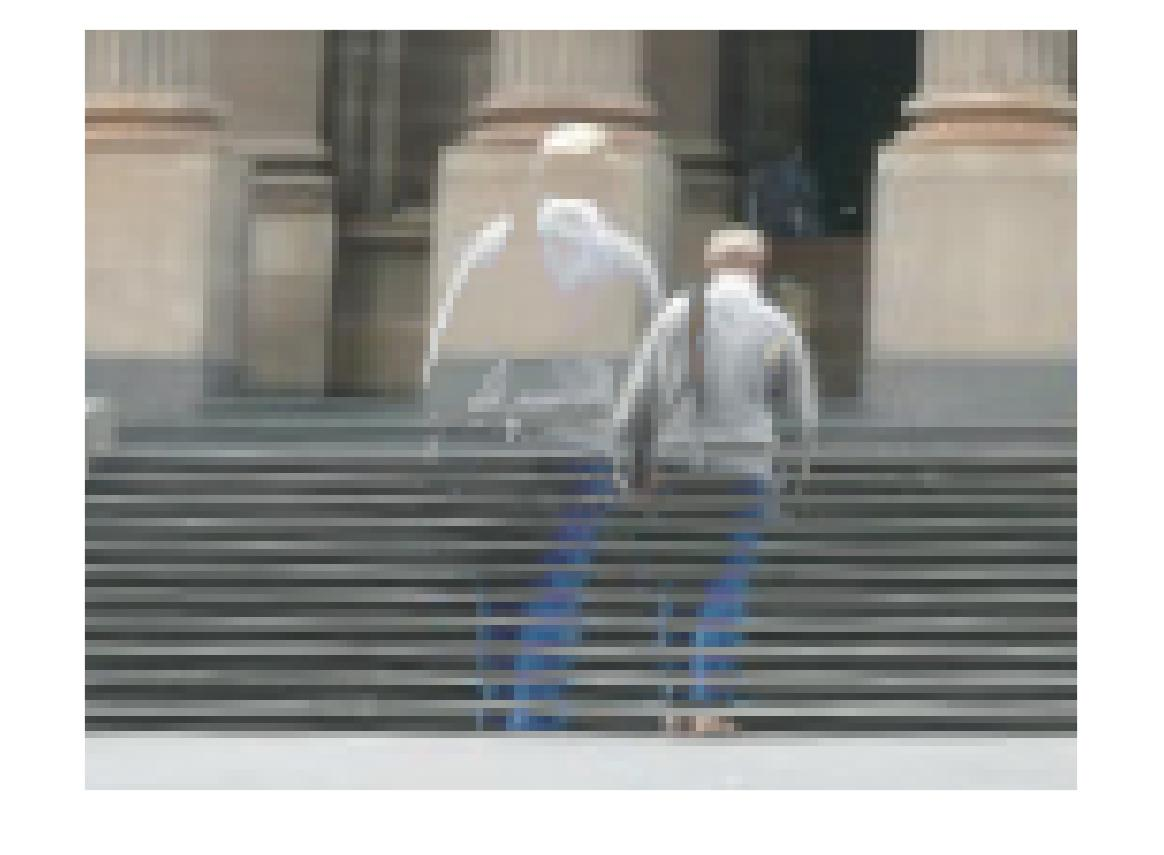
\includegraphics[width=0.5\linewidth]{img/set1_ghost2}
    \caption{The problem with merging images}
    \label{fig_ghost}
\end{figure}

\end{document}